\documentclass[12pt,twoside,a4paper]{article}
\usepackage{hyperref}
\usepackage{graphicx}
\usepackage[T1]{fontenc}
\usepackage[utf8]{inputenc}
\usepackage{enumitem}
\usepackage{array,tabularx}

\setlist[enumerate,1]{labelindent=0pt, leftmargin=*}
\pagestyle{empty}

\newcolumntype{P}{>{\centering\arraybackslash}p{0.75cm}}
\newcolumntype{L}{>{\raggedright\arraybackslash}m{0.2\textwidth}}
\newcolumntype{R}{>{\raggedleft\arraybackslash}m{0.2\textwidth}}

\newcommand{\usetbl}{%
  \begin{tabular}{@{}|*7{P|}@{}}
    \hline
    0 & 1 & 2 & 3 & 4 & 5 & 6 \\
    \hline
  \end{tabular}
}

\newcommand\prop[1]{%
  \item
  \parbox[t]{0.25\textwidth}{#1}%
  \qquad
  \parbox[t]{0.5\textwidth}{\usetbl}%
}

\graphicspath{{images/}}

\hypersetup{
    colorlinks=true,
    linkcolor=blue,
    filecolor=magenta,
    urlcolor=cyan,
    citecolor=black,
}

\begin{document}
% Header-Make sure you update this information!!!!
\noindent
\large
\textbf{BIRADS Survey} \hfill \textbf{Institution} \\
\normalsize
\hyperlink{https://github.com/MIMBCD-UI/prototype-single-modality}{Single-Modality Prototype} \hfill Universidade de Lisboa (ULisboa) \\
\hyperlink{https://github.com/MIMBCD-UI/prototype-multi-modality}{Multi-Modality Prototype} \hfill Instituto Superior T\'{e}cnico \\

%%%%%%%%%%%%%%%%%%%%%%%%%%%%%%%%%%%%%%%%%%%%%%%%%%%
%                                                 %
%                     SECTION                     %
%                                                 %
%%%%%%%%%%%%%%%%%%%%%%%%%%%%%%%%%%%%%%%%%%%%%%%%%%%

\hspace*{0.55\textwidth}%
\begin{tabularx}{0.5\textwidth}{@{}LR@{}}
\textbf{} & \textbf{} \\
\textbf{} & \textbf{} \\
\end{tabularx}

{\renewcommand\labelitemi{}
\begin{itemize}
\prop{BIRADS:}
\end{itemize}
}
%%%%%%%%%%%%%%%%%%%%%%%%%%%%%%%%%%%%%%%%%%%%%%%%%%%
%                                                 %
%                     IMAGE                       %
%                                                 %
%%%%%%%%%%%%%%%%%%%%%%%%%%%%%%%%%%%%%%%%%%%%%%%%%%%

\begin{figure}[h]
\center
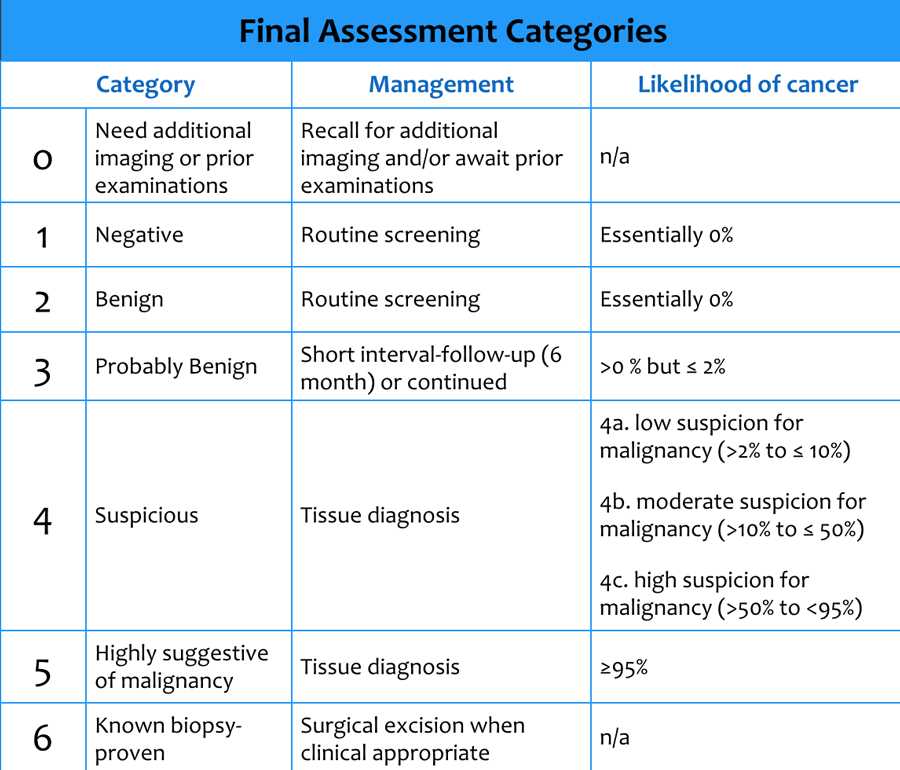
\includegraphics[width=\textwidth]{birads}
\caption{BIRADS Final Assessment Categories.}
\label{fig:birads}
\end{figure}

\clearpage

%%%%%%%%%%%%%%%%%%%%%%%%%%%%%%%%%%%%%%%%%%%%%%%%%%%
%                                                 %
%                     SECTION                     %
%                                                 %
%%%%%%%%%%%%%%%%%%%%%%%%%%%%%%%%%%%%%%%%%%%%%%%%%%%

\section*{Information}

The following information describes the detailed data regarding the user tests of the research work. The data will therefore be important to the BIRADS analysis.

\vspace{1cm}

\textbf{Participant Name} \hfill \textbf{Date}

\vspace{2.5cm}

\textbf{Test} \hfill \textbf{Location}

\vspace{2.5cm}

\textbf{Prototype} \hfill \textbf{Version}

\vfill

%%%%%%%%%%%%%%%%%%%%%%%%%%%%%%%%%%%%%%%%%%%%%%%%%%%
%                                                 %
%                     SECTION                     %
%                                                 %
%%%%%%%%%%%%%%%%%%%%%%%%%%%%%%%%%%%%%%%%%%%%%%%%%%%

\section*{Support}

\hfill

List of sponsors, honers and donors:

\hfill

%%%%%%%%%%%%%%%%%%%%%%%%%%%%%%%%%%%%%%%%%%%%%%%%%%%

\hfill


\includegraphics[width=0.25\textwidth]{logo} \hfill 
\includegraphics[width=0.25\textwidth]{logo} \hfill 
\includegraphics[width=0.25\textwidth]{logo}


\includegraphics[width=0.25\textwidth]{logo} \hfill 
\includegraphics[width=0.25\textwidth]{logo} \hfill 
\includegraphics[width=0.25\textwidth]{logo}

\hfill

%%%%%%%%%%%%%%%%%%%%%%%%%%%%%%%%%%%%%%%%%%%%%%%%%%%

\end{document}